% !TeX encoding = UTF-8
% !TeX spellcheck = es_ES
% !TeX root = Thermal.tex
%!TEX root=Thermal.tex

\documentclass[spanish]{DccDiyTools/DccDiyTools}
\usepackage[spanish]{babel}
\usepackage[
type={CC},
modifier={by-sa},
version={4.0},
]{doclicense}

\usepackage[]{DccDiyTools/DccDiyToolsPics}
\usepackage[]{DccDiyTools/DccDiyToolsComponentTables}


\title{Termica de Componentes}
\subtitle{Informacion de calculos termicos}
\author{Daniel Vilas}
\date{Julio 2022}

\dbHeaderTitle{Termica de Componentes}
\dbType{M}
\dbDate{22}
\dbCode{002}
\dbStatus{Draft}
\dbVersion{0.1}
%\tikzset{
    pics/SmallBoard/.style={
      code = {
        % \draw [step=0.1,very thin, yellow] (-2,-1) grid (2,1);
        % \draw [step=0.5,very thin, red] (-2,-1) grid (2,1);
        % \draw [very thin, green] (-2,-1) grid (2,1);
        \node[inner sep=0pt] at (0,0)
        {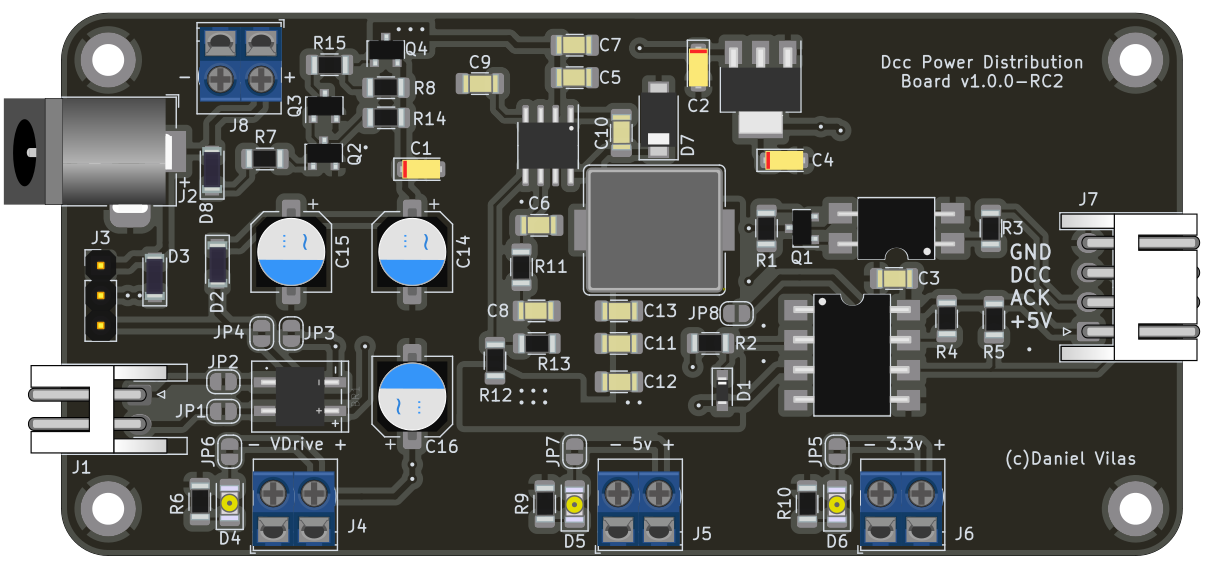
\includegraphics[scale=0.25]{images/front.png}};  


        \node[](-jack) at (-1.35,0.278) {};
        \node[](-terminal) at (-.8,0.65) {};
    }}
}

\tikzset{
    pics/WallAc/.style={
      code = {
    \begin{scope}[shift={(0.25,0)}]
        % \draw [step=0.1,very thin, yellow] (-2,-2) grid (2,2);
        % \draw [step=0.5,very thin, red] (-2,-2) grid (2,2);
        % \draw [very thin, green] (-2,-2) grid (2,2);
        % Mains lead
        \draw[line width=2pt,cap=round, lightgray] (0.05,-0.21) -- (0.05,-0.45);
        \draw[line width=2pt,cap=round, lightgray] (0.275,-0.21) -- (0.275,-0.45);
        % Relief and out cable
        \draw[line width=2pt,cap=round] (-0.5,0.25) -- (-1,0.25);
        \draw[line width=2pt,cap=round,black!75] (-0.55,0.35)--(-0.55,0.15);
        \draw[line width=2pt,cap=round,black!75] (-0.63,0.325)--(-0.63,0.175);
        \draw[line width=2pt,cap=round,black!75] (-0.71,0.3)--(-0.71,0.2);
        \draw[line width=2pt,cap=round,black!75] (-0.79,0.275)--(-0.79,0.225);
        \draw[line width=2pt,cap=round,black!75] (-0.87,0.275)--(-0.87,0.225);

        \draw[line width=2pt,rounded corners=1pt,fill=black!75] (-0.5,0) rectangle +(1,0.5);
        \draw[line width=2pt,rounded corners=1pt,fill=black!65] (-0.1,0) rectangle +(0.5,-0.2);
        % \draw[line width=2pt,cap=round, gray] (0.05,-0.21) -- (0.05,-0.45);
        % \draw[line width=2pt,cap=round,gray] (0.275,-0.21) -- (0.275,-0.45);

        \node[white,scale=0.5] at (0,0.25) {DC Wall};
        \node[](-jack) at (-1.1,0.25) {};
        \node[](-mains) at (.1625,-0.55) {};
    \end{scope}
    }}
}



\begin{document}
\maketitle
\newpage
\section{Introduccion}
% !TeX encoding = UTF-8
% !TeX spellcheck = es_ES
% !TeX root = CBus.tex
%!TEX root=CBus.tex
C-Bus es un standard LCB usado y promocionado por MERG\copyright. A bajo nivel utiliza un Bus CAN como transporte fisico de datos entre modulos (electronicos).

La idea de despligue es usar una topolgia de bus:
\begin{figure}[H]
    \centering
    \begin{tikzpicture}
        %\draw [very thin, green]  (-6,-3) grid (6,3);
        \node at (-6,3) [rectangle,draw,align=left] (ps) {Previous\\Segment};
        \node at (6,3) [rectangle,draw,align=left] (ns) {Next\\Segment};
        
        \node at (-2.75,0) [rectangle,draw,align=left] (d1) {Modulo 1};
        \node at (0,0) [rectangle,draw,align=left] (d2) {Modulo 2};
        \node at (2.75,0) [rectangle,draw,align=left] (d3) {Modulo ...};

        \draw [line width=2, blue] (-4,3) -- (-4,0) --(d1.west);
        \draw [line width=2, blue] (-1.25,3) -- (-1.25,0) --(d2.west);
        \draw [line width=2, blue] (1.5,3) -- (1.5,0) --(d3.west);

        \draw [line width=5] (ps.east) -- (ns.west);
    \end{tikzpicture}
    \caption{C-Bus Segmento}
    \label{fig:cBusSegment}
\end{figure}

Al final de un segmento puede haber otro segmento, un repetidor, un convertidor a Ethernet,\dots.
Desde el bus a los dispositivos es necesario tener un latiguillo.




\newpage
\section{Calculos generales}
% !TeX encoding = UTF-8
% !TeX spellcheck = es_ES
% !TeX root = Thermal.tex
%!TEX root=Thermal.tex

La forma de modelar/estimar que temperatura alcanzara el silicio en un chip es considerar
la potencia que disipa como una fuente de corriente y el camino que tiene hasta el aire como
una resistencia modelo simplificado(a)\ref{fig:ThermalEquivalent}:

\begin{figure}[H]
    \centering
    % !TeX encoding = UTF-8
% !TeX spellcheck = es_ES
% !TeX root = ../Thermal.tex
%!TEX root=../Thermal.tex

\begin{tikzpicture}[american]
    %\draw (0,0) circle[radius=1pt];
    \begin{scope}[shift={(-5,0)}]
        %\draw (0,0) circle[radius=1pt];
        %\draw (-2.5,-3.5) rectangle +(5,7);
        
        \draw (-2,2.5) to[isource, l=$W$ ] (0.5,2.5)
            node[right,red]{$T_j$} 
            to[R, l2=$R_{thJA}$ and $\si{\degree\kelvin\per\watt}$] (0.5,-0)
            node[right,red]{$T_{amb}$} 
            to[vsource=$T_a$] (0.5,-2.5)
            node[right,red]{$\SI{0}{\celsius}$} 
            node[ground](gnd){};
        \node at(0,-3.5) {a) Simplificado};
    \end{scope}


    \begin{scope}[shift={(-0,0)}]
        %\draw (0,0) circle[radius=1pt];
        %\draw (-2.5,-4.75) rectangle +(5,9.5);
        
        \draw (-2,3.75) to[isource, l=$W$ ] (0.5,3.75)
            node[right,red]{$T_j$} 
            to[R, l2=$R_{thJC}$ and $\si{\degree\kelvin\per\watt}$] (0.5,1.25)
            node[right,red]{$T_{case}$} 
            to[R, l2=$R_{thCA}$ and $\si{\degree\kelvin\per\watt}$] (0.5,-1.25)
            node[right,red]{$T_{amb}$} 
            to[vsource=$T_a$] (0.5,-3.75)
            node[right,red]{$\SI{0}{\celsius}$} 
            node[ground](gnd){};
        \node at(0,-4.75) {b) Normal};
    \end{scope}

    \begin{scope}[shift={(5,0)}]
        %\draw (0,0) circle[radius=1pt];
        %\draw (-2.5,-3.5) rectangle +(5,7);
        
        \draw (-2,3.75) to[isource, l=$W$ ] (0.5,3.75)
            node[right,red]{$T_j \leq \SI{125}{\celsius}$} 
            to[R, l2=$R_{thHS}$ and $\si{\degree\kelvin\per\watt}$] (0.5,1.25)
            node[right,red]{$T_{case} \leq \SI{100}{\celsius}$} 
            to[R, l2=$R_{thJC}$ and $\si{\degree\kelvin\per\watt}$] (0.5,-1.25)
        
            node[right,red]{$T_{amb}\approx \SI{25}{\celsius}$} 
            to[vsource=$T_a$] (0.5,-3.75)
            node[right,red]{$\SI{0}{\celsius}$} 
            node[ground](gnd){};
        \node at(0,-4.75) {c) Usable};
    \end{scope}

\end{tikzpicture}

    \caption{Circuito Equivalente}
    \label{fig:ThermalEquivalent}
\end{figure}

En la practica se puede modelar como dos resistencias, una $R_{thJC}$ :
Junction\sidenote{El silicio} a la case\sidenote{Carcasa} y $R_{thCA}$ de la 
carcasa al ambiente, tal y como se representa en el caso (b) \ref{fig:ThermalEquivalent}.
En este modelo es importante mantener la temperatura del silicio $T_j$ por debajo de
$\SI{125}{\celsius}$ lo que se corresponde con $T_c=\SI{100}{\celsius}$ en la carcasa.
En la realidad, el modelo es más complejo, con resistencias en paralelo segun el dispador
que se ponga, pero se simplifica por la diferencia valores y se puede ignorar $R_{thCA}$
por $R_{thHS}$ del disipador\sidenote{HeatSink}.

Estos modelos los podemos complicar un poco más\sidenote{Acercandose más
a la realidad}, dependiendo de si usamos un dispador sobre un componente o 
usamos la propia PCB como disipador. En cuyo caso la resitencia termica es
de $\SI{100}{\degree\kelvin/\square{inch}}$ o $\SI{645.16}{\degree\kelvin/\square\cm}$.
Aunque estos valores dependeran en gran medida de los materiales usados en la 
fabricacion de la PCB.


\begin{figure}[H]
    \centering
    % !TeX encoding = UTF-8
% !TeX spellcheck = es_ES
% !TeX root = ../Thermal.tex
%!TEX root=../Thermal.tex

\begin{tikzpicture}[american]
    %\draw (0,0) circle[radius=1pt];
    \begin{scope}[shift={(-3,0)}]
        %\draw (0,0) circle[radius=1pt];
        %\draw (-3.25,-5.5) rectangle +(6.5,11);
			
			\draw (-2.75,4.5)
				to[isource, l=$W$ ] ++(2.5,0) 
				node [red, right] {$T_{j}$}
				to [R,l=$R_{thJC}$] ++(0,-2.5) 
					coordinate(TC)
				node[red,left]{$T_{case}$}
				to [R,l=$R_{thCA}$] ++ (0,-4)
					coordinate(TA)
				node[red,left]{$T_{amb}$}
				to[vsource,v=$T_{amb}$] ++(0,-2.5)
				node[ground]{};
			\draw (TC) to[short,*-] ++(2,0)
				to[R,l=$R_{thS}$] ++(0,-2.)
				to[R,l=$R_{thHS}$] ++(0,-2.)
				to[short,-*](TA);
			\node[] at (0,-5.5){a) Componente TH};
     \end{scope}
	  \begin{scope}[shift={(5,0)}]
			%\draw (-5.25,-5.5) rectangle +(10.5,11);
			
			\draw (-4.75,4.5)
				to[isource, l=$W$ ] ++(2.5,0)
					coordinate(TJ) 
				node [red, above] {$T_{j}$}
				to [R,l=$R_{thJC}$] ++(0,-2.5) 
					coordinate(TC)
				node[red,left]{$T_{case}$}
				to [R,l=$R_{thCA}$] ++ (0,-4)
					coordinate(TA)
				node[red,left]{$T_{amb}$}
				to[vsource,v=$T_{amb}$] ++(0,-2.5)
				node[ground]{};
			\draw (TJ) to[short,*-] ++(2.5,0)
				to[R,l=$R_{thJL}$] ++(0,-2.5)
					coordinate(TL)
					node[red,right]{$T_l$}
				to[R,l=$R_{thLC}$] (TC);
			\draw (TL) to [R,l=$R_{thS}$] ++ (0,-2)
					coordinate(Ttop)
					node[red,left]{$T_{top}$}
				to[R,l=$R_{thTopPcb}$]++(0,-2)
				to[short,-*](TA);
			\draw (Ttop) to [vsource,v_=$\SI{10}{\degree\kelvin}$] ++(3,0)
			node[red,right ]{$T_{bott}$}
			to[R,l=$R_{thBottPcb}$] ++(0,-2)
			to[short,-*] (TA)
			;

			%\draw (TC) to[short,*-] ++(2,0)
			%	to[R,l=$R_{thS}$] ++(0,-2.)
			%	to[R,l=$R_{thHS}$] ++(0,-2.)
			%	to[short,-*](TA);
			
			\node[] at (0,-5.5){b) SMD usando PCB como Disipador};
     \end{scope}

\end{tikzpicture}
    \caption{Diseño más complejo}
    \label{fig:ThermalEquivFull}
\end{figure}

Ahora es momento de implificar el circutito teniendo en cuenta la regla del 10
\sidenote{En realidad depende de la tolerancia}. pudiendo eliminar una resistencia
si hay otra 10 veces mas grande o pequeña segun sea el caso:
\begin{itemize}
    \item \textbf{En serie}: Si $R_p$ es 10 menor que $R_g$, podemos eliminarla puesto que 
    $R_p$ se esconderia en la tolerancia de $R_g$.

    En nuestro caso sucede con $R_{thS}$,$R_{thSn}$, siendo, repsecivamente, estas la pasta
    termica que se pone entre un chip y el dispador, y el estaño que une un pad a la PCB.
    ambas cercanas a \SI{1}{\degree\kelvin/\watt}
    \item \textbf{En paralelo}: Si $R_g$ es los suficientemente grande, su valor se esconderia
    en la tolerancia de $R_p$, por lo que puede eleminarse. Para el calculo de temperaturas, donde nuestro
    origen es una fuente de calor representada como fuente de corriente, lo que hace es "<robar">
    un poco de corriente a $R_p$, por lo que al eleminar $R_g$ tendremos un error al alza. 
    Habiendo calculado una temperatura superior a la real, y si esta es segura, la real tambien.
    
    Asi pues con un disipador correcto ($R_{thHS}$, o la red que representa la PCB), podremos quitar
    $R_{thCA}$.
    \item \textbf{Otras}: Como la conexion en delta, se pueden llegar a simplifcar
    pensando en cuanta corriente se llevan, pero lo normal es que los fabricantes ya
    hayan echo los calculos y no sean necesarios. Como el es el caso de $R_{thLC}$.    
\end{itemize}

\newpage
\section{Indice}
\tableofcontents

\listoffigures
\listoftables

\bibliographystyle{unsrt}
\bibliography{bibliography}

\end{document}